\documentclass[a4paper, 12pt]{article}

\usepackage{hyperref}
\usepackage[warn]{mathtext}
\usepackage[utf8]{inputenc}
\usepackage[T2A]{fontenc}
\usepackage[english,russian]{babel}
\usepackage{multirow}
\usepackage{float}
\restylefloat{table}
\usepackage{amsmath,amsfonts,amssymb,amsthm,mathtools}
\usepackage{indentfirst}
\DeclareSymbolFont{T2Aletters}{T2A}{cmr}{m}{it}
\usepackage{ gensymb }
\mathtoolsset{showonlyrefs=true}
\usepackage{euscript}
\usepackage{mathrsfs}
\usepackage[left=2cm,right=2cm,top=2cm,bottom=2cm]{geometry}
\usepackage{graphicx}
\usepackage{wrapfig}
\usepackage[rgb]{xcolor}
\hypersetup{
colorlinks=true,
urlcolor=blue
}
\usepackage{tikz}

\title{Лабораторная работа}
\author{Гисич Арсений Б03-102}
\date{2023}

\begin{document}

	\begin{center}
		{\large МОСКОВСКИЙ ФИЗИКО-ТЕХНИЧЕСКИЙ ИНСТИТУТ (НАЦИОНАЛЬНЫЙ ИССЛЕДОВАТЕЛЬСКИЙ УНИВЕРСИТЕТ)}
	\end{center}
	\vspace{5 cm}
	{\Large
		\begin{center}
			{\bf Лабораторная работа 4.3.3}\\[0.2 cm]
			Исследование разрешающей способности микроскопа \\ методом Аббе
		\end{center}
	}
	\vspace{4 cm}
	\begin{flushright}
		{\Large Выполнил: \\
			\vspace{0.2 cm}
			Гисич Арсений \\
			\vspace{0.2 cm}
			Б03-102 \\}
	\end{flushright}
	\vspace{8 cm}
	\begin{center}
		Долгопрудный\\[0.1 cm]
		2023
	\end{center}
\thispagestyle{empty}

\section{Аннотация}

В данной работе был определён период сеток сначала по их спектру на удалённом экране, затем по увеличенному с помощью модели микроскопа изображению сеток на экране и, наконец, по результатам измерения разрешающей способности микроскопа; наблюдались явления саморепродукции, пространственной фильтрации и мультиплицирования.

\section{Теоретические сведения}

\textit{Разрешающей способностью оптического прибора} называют минимальное расстояние $l_{\text{min}}$ между двумя точками в пространстве предметов, которое прибор может разрешить. Если наблюдения с помощью микроскопа ведутся при внешнем освещении, то, как правило, различные точки предмета рассеивают когерентные волны. Теория разрешающей способности для случая освещаемых объектов была разработана Аббе.

	Рассмотрим когерентно освещенный объект, наблюдаемый в объектив микроскопа. Минимальное разрешаемое объективом расстояние определяется условием
	\begin{equation}
		\label{min}
		l_{\text{min}} \approx \frac{\lambda}{\sin A} \approx \frac{\lambda}{D/2f},
	\end{equation}
	где $A$ --- апертурный угол микроскопа, $D$ --- диаметр диафрагмы. При этом диафрагма, расположенная симметрично, пропускает нулевой и $\pm 1$ дифракционные максимумы.
	
	В нашей работе применяется двумерная решётка --- сетка. В таком случае главные максимумы возникают тогда, когда одновременно выполняются условия:
	\begin{equation}
		\label{system}
		\begin{cases}
			d \sin \theta_x = m_x \lambda, \\
			d \sin \theta_y = m_y \lambda,
		\end{cases}
	\end{equation}
	где $m_x$ и $m_y$ --- целые числа, характеризующие порядки дифракционных максимумов, $\theta_x$ и $\theta_y$ --- направления на главные дифракционные максимумы в горизонтальное и вертикальной плоскостях соответственно.
	
	Максимумы, удовлетворяющие условию $\theta_x, \theta_y < A$, создают в задней фокальной плоскости $F$ объектива картину дифракции Фраунгофера (рис.~\ref{ris:max}) --- первичное изображение.
	\begin{figure}[H]
		\center{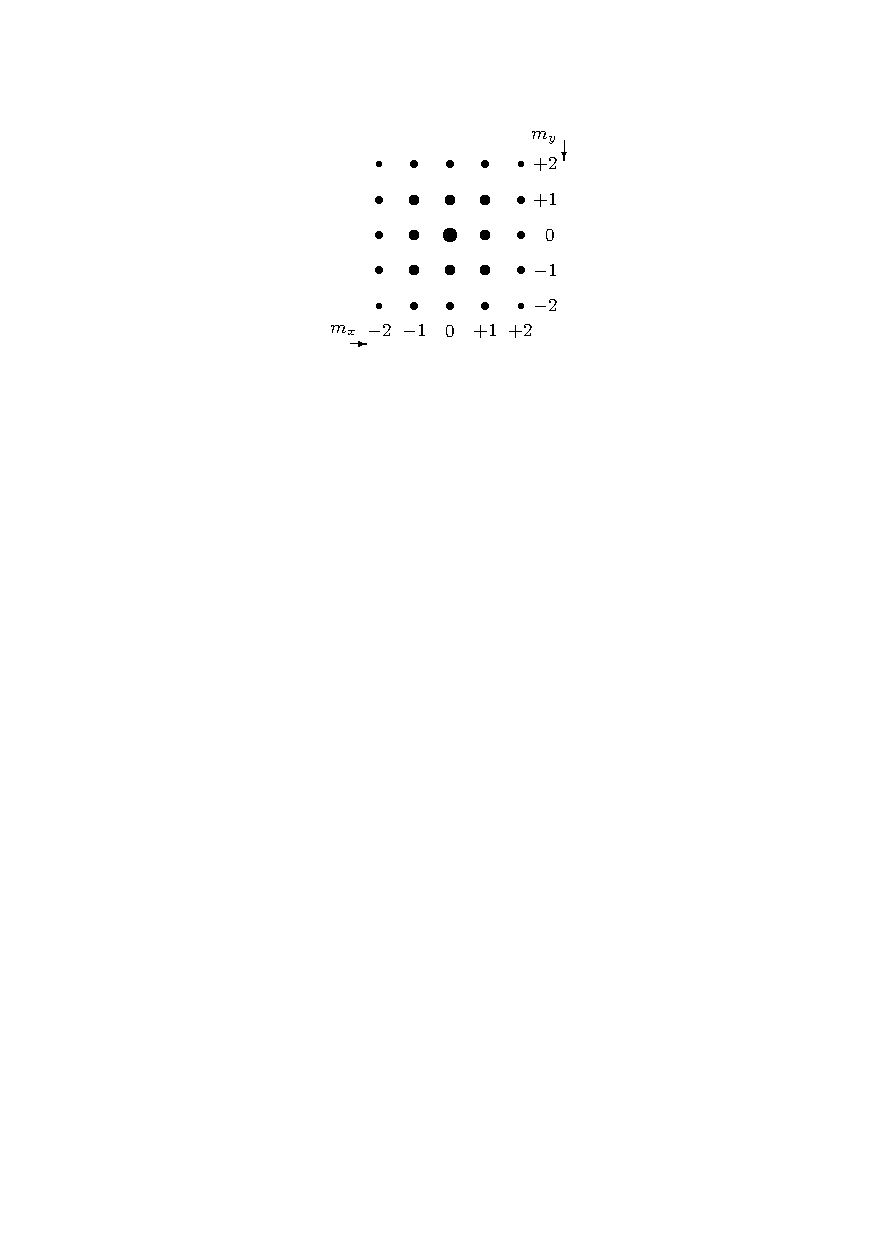
\includegraphics[scale=1.2]{max.pdf}}
		\caption{Дифракция Фраунгофера на двумерной решётке (сетке). Максимумы изображены кружками, размеры которых характеризуют интенсивности.}
		\label{ris:max}
	\end{figure}
	
	Если теперь поместить в фокальной плоскости щель так, чтобы через неё проходили дифракционные максимумы с $m_x = 0$ и $m_y =0, \pm 1, \pm 2, ...$ (с $m_y = 0$ и $m_x =0, \pm 1, \pm 2, ...$), то в плоскости $P_2$ получится изображение решётки с горизонтальными (вертикальными) штрихами. Таким образом можно продемонстрировать явление \textit{пространственной фильтрации} --- выделение различных структур в изображении.

\section{Методика измерений}

Схема модели проекционного микроскопа приведена на рис.~\ref{ris:ustanovka}. Предметом служат сетки, расположенные в штативе.
	\begin{figure}[H]
		\center{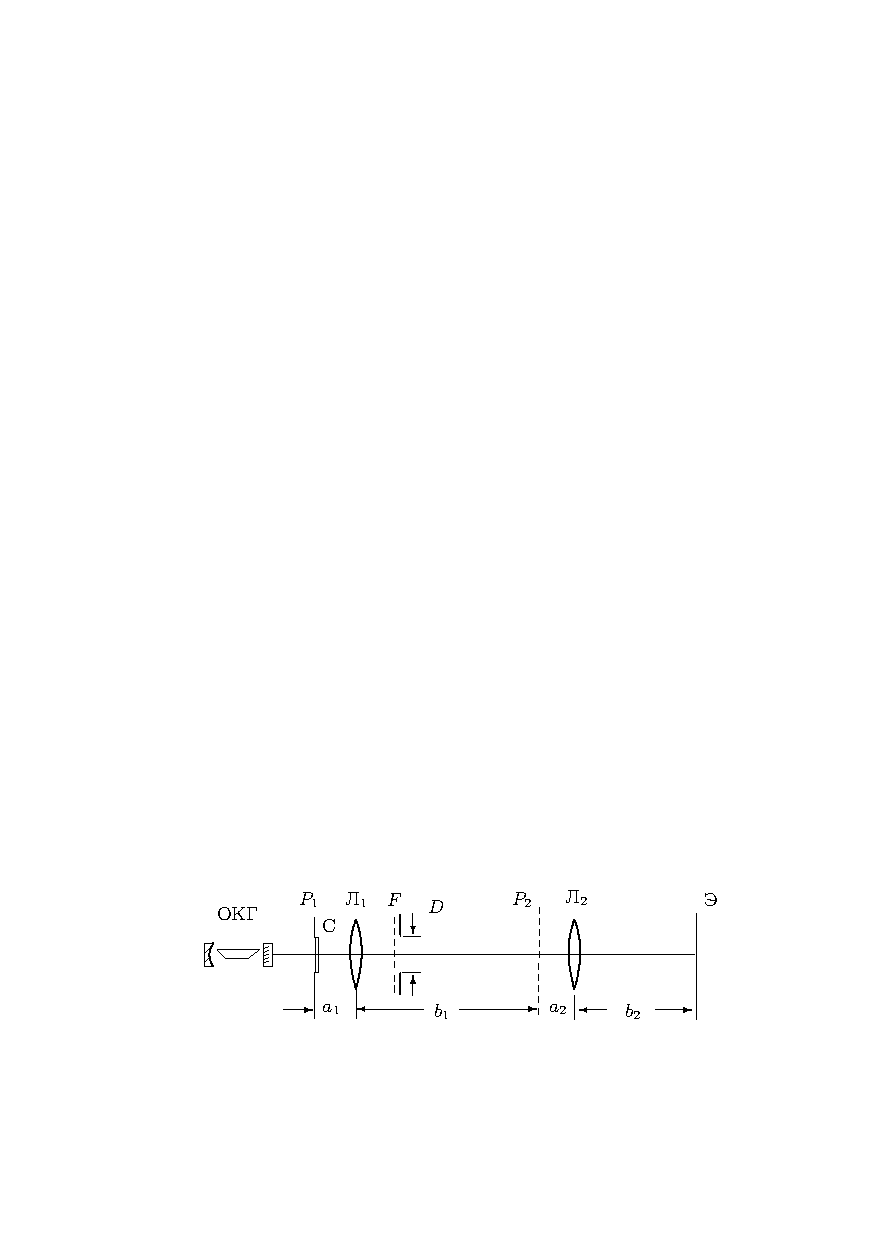
\includegraphics[scale=1.2]{ustanovka.pdf}}
		\caption{Схема экспериментальной установки -- модель проекционного микроскопа.}
		\label{ris:ustanovka}
	\end{figure}
	Изображение сетки периодически повторяется --- \textit{репродуцируется} --- в пространстве между сеткой и первой линзой. Для выделения геометрического изображения среди множества репродуцированных изображений сетки на одну из сеток наложена тонкая проволока, то есть непериодический объект, изображение которого не репродуцируется.
  	
\section{Используемое оборудование}

\begin{enumerate}
    \item лазер;
	\item кассета с набором сеток разного периода;
	\item линзы;
	\item щель с микрометрическим винтом;
	\item оптический стол с набором рейтеров и крепёжных винтов;
	\item экран;
    \item линейка.
\end{enumerate}

\section{Результаты измерений и обработка данных}

Параметры установки:
\begin{description}
\item{} $F_1 = 110~мм$
\item{} $F_2 = 25~мм$
\item{} $\lambda = 532~нм$
\end{description}

\subsection{Определение периода решёток по их пространственному спектру}

Установим кассету с двумерными решётками вблизи выходного окна лазера. Измерения расстояния между соседними (горизонтальными и вертикальными) дифракционными максимумами и периода решётки представлены в таб.~\ref{tab1}. Из формулы (\ref{system}) выразим $d = m \lambda / \sin \theta$, причем $\sin \theta \approx (l/n)/L$ и $m = 1$, где $l$ --- расстояние между удалёнными друг от друга максимумами.

\begin{table}[h!]
\begin{center}
\begin{tabular}{|c|c|c|c|}
\hline 
Номер решётки & $l$, см & $d$, мкм  \\ 
\hline 
1 & $6,3\pm0,1$ & $9,9\pm0,2$ \\ 
\hline 
2 & $2,5\pm0,1$ & $25,0\pm1,0$ \\ 
\hline 
3 & $1,3\pm0,1$ & $48,2\pm3,7$ \\ 
\hline  
\end{tabular} 
\end{center}
\caption{Результаты измерений периода решёток по их дифракционной картине}
\label{tab1}
\end{table}

Расстояние от сетки до экрана $H = 117,7\pm1~см$.

\subsection{Определение периода решёток по изображению, увеличенному с помощью модели микроскопа}

Соберём модель проекционного микроскопа (рис.~\ref{ris:ustanovka}). Для того, чтобы выделить изображение сетки, соответствующее законам геометрической оптики, найдём резкое изображение проволочки, расположенной на сетках.

\begin{figure}[h!]
		\begin{minipage}[h!]{0.3\linewidth}
			\center{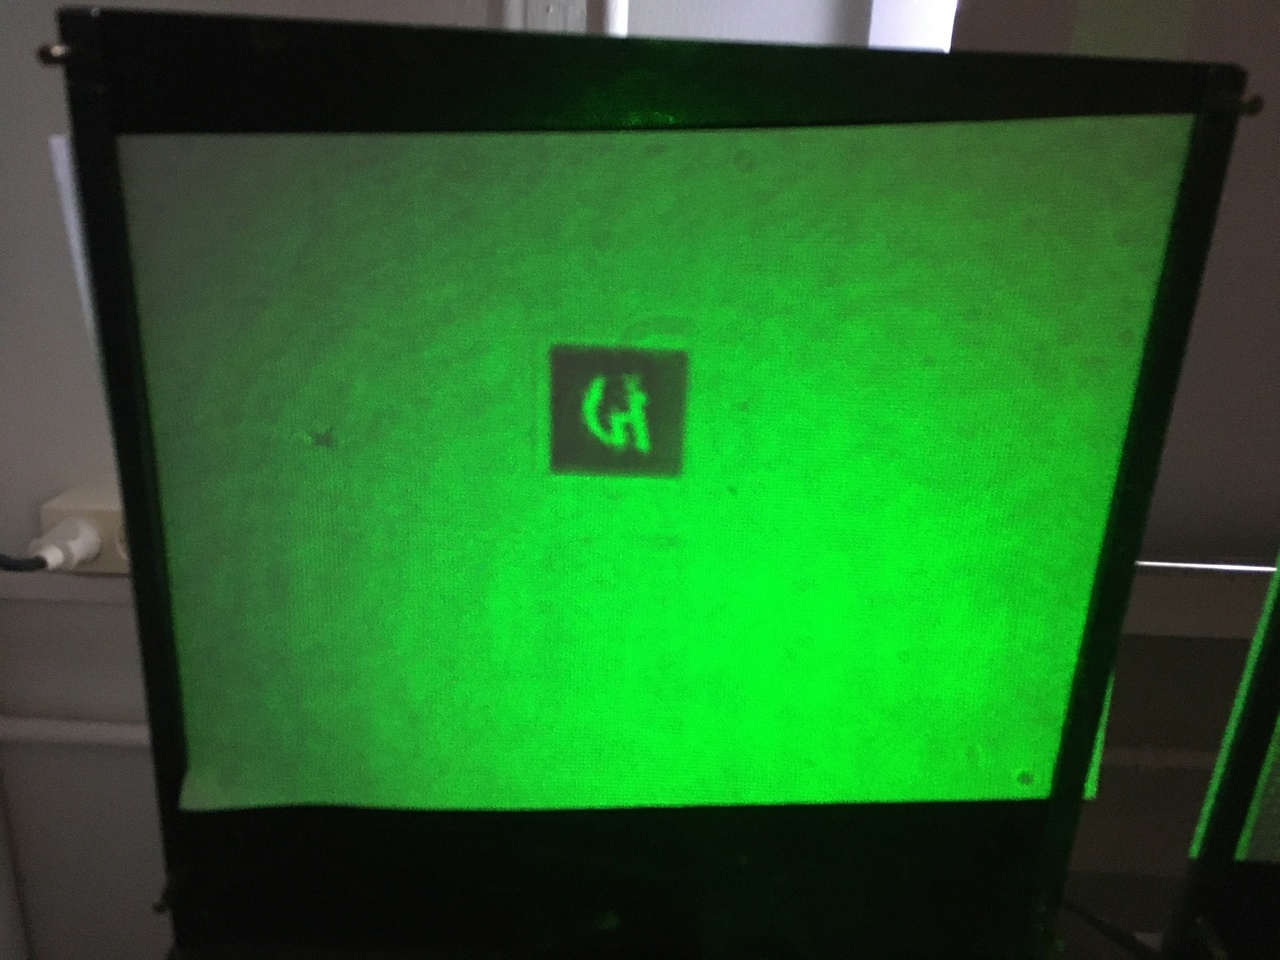
\includegraphics[width=1\linewidth]{grid1.jpg}}
		\end{minipage}
		\hfill
		\begin{minipage}[h!]{0.3\linewidth}
			\center{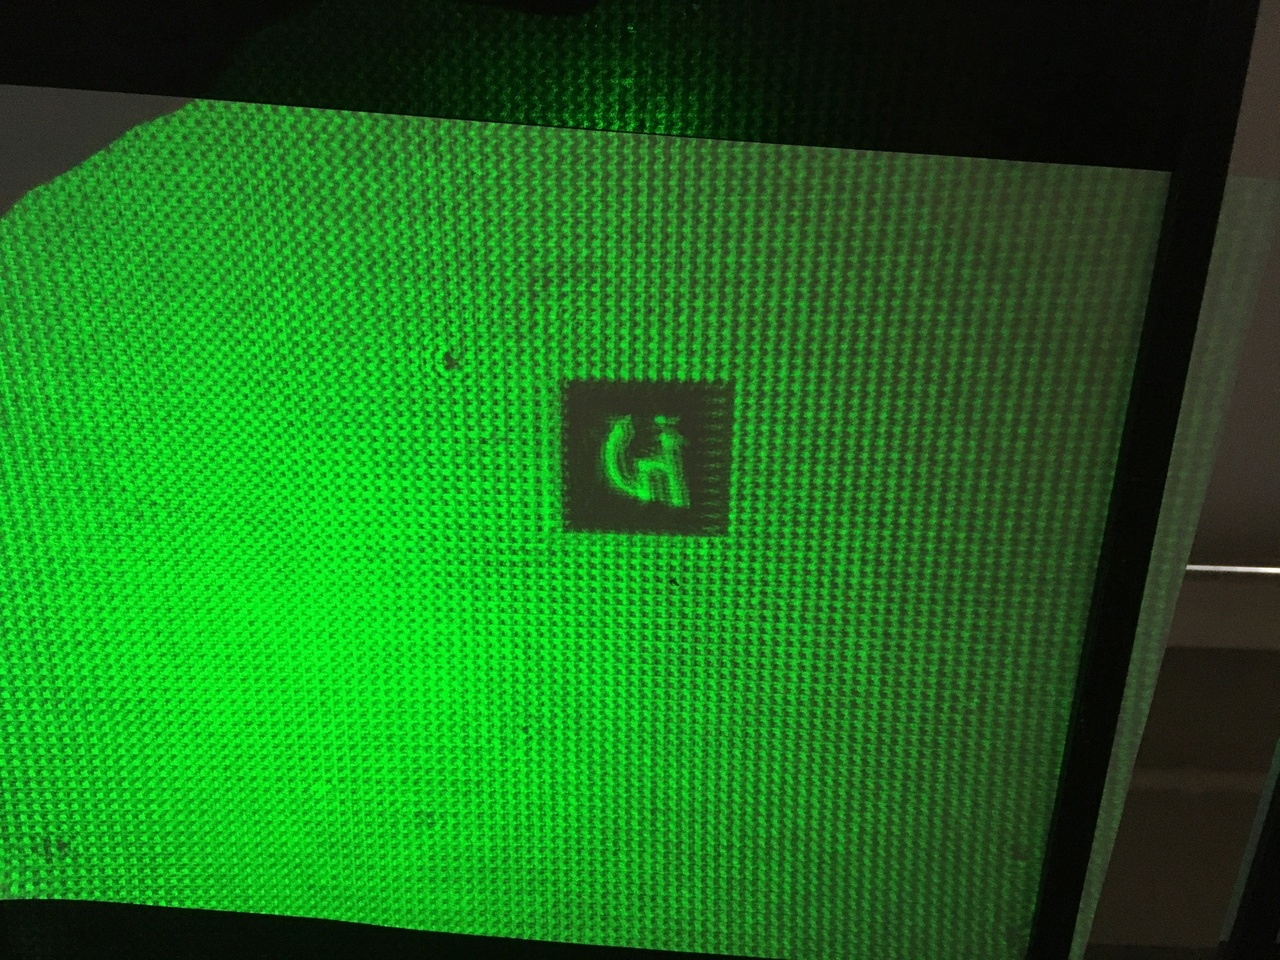
\includegraphics[width=1\linewidth]{grid2.jpg}}
		\end{minipage}
		\hfill
		\begin{minipage}[h!]{0.3\linewidth}
			\center{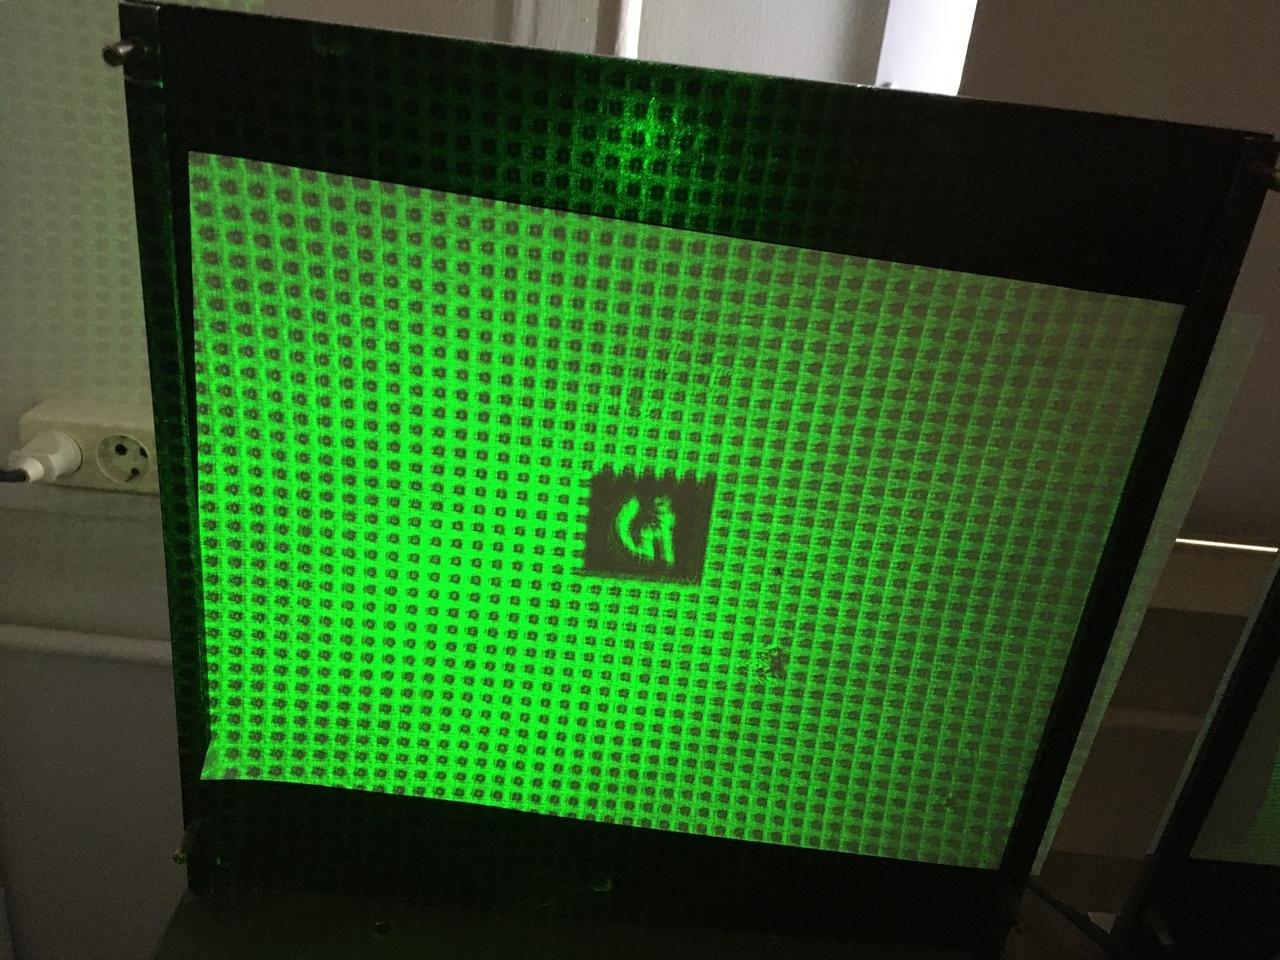
\includegraphics[width=1\linewidth]{grid3.jpg}}
		\end{minipage}
		\hfill
		\caption{Изображения дифракционных решёток}
		\label{fig:grid_images}
\end{figure}

Полученные значения расстояний:
\begin{description}
\item{} $a_1 = 15\pm1~см$
\item{} $b_2 = 63\pm1~см$
\item{} $(b_1 + a_2) = 61,5\pm1~см$
\end{description}

Результаты измерения периода дифракционной решётки методом изображения представлены в таб.~\ref{tab2}. Периоды решёток определяются по формуле $d = l/Г$, где \newline $Г = \frac{b_1 b_2}{a_1 a_2} = 510$ --- увеличение оптической системы.

\begin{table}[h!]
\begin{center}
\begin{tabular}{|c|c|c|c|}
\hline 
Номер решётки & $l$, см & $d$, мкм \\ 
\hline 
1 & $0,14$ & $2,8$ \\ 
\hline 
2 & $0,33$ & $6,5$ \\ 
\hline 
3 & $0,6$ & $11,8$ \\ 
\hline  
\end{tabular} 
\end{center}
\caption{Результаты измерений периода решёток по их изображению в модели микроскопа}
\label{tab2}
\end{table}

\newpage

\subsection{Определение периодов решёток по оценке разрешающей способности микроскопа}

Поместим щелевую диафрагму с микрометрическим винтом в фокальную плоскость F линзы Л$_1$. Из формулы~(\ref{min}) следует, что $d =~2\lambda f_1 / D$. Результаты измерений представлены в таб.~\ref{tab3}.

\begin{table}[h!]
\begin{center}
\begin{tabular}{|c|c|c|c|}
\hline 
Номер решётки & $D$, мкм & $d$, мкм \\ 
\hline 
1 & $6760$ & $17,3$ \\ 
\hline 
2 & $3200$ & $36,6$ \\ 
\hline 
3 & $1120$ & $104,5$ \\ 
\hline  
\end{tabular} 
\end{center}
\caption{Результаты измерений периода решёток по оценке разрешающей способности микроскопа}
\label{tab3}
\end{table}

\subsection{Сравнение результатов}

Результаты измерения периодов дифракционных решёток различными способами представлены в таб.~\ref{tab:all}.

\begin{table}[h!]
\begin{center}
\begin{tabular}{|c|c|c|c|}
\hline 
Номер решётки & $d_1$, мкм & $d_2$, мкм & $d_3$, мкм \\ 
\hline 
1 & $9,9$ & $2,8$ & $17,3$ \\ 
\hline 
2 & $25,0$ & $6,5$ & $36,6$ \\ 
\hline 
3 & $48,2$ & $11,8$ & $104,5$ \\ 
\hline  
\end{tabular} 
\end{center}
\caption{Результаты измерений периода решёток различными способами}
\label{tab:all}
\end{table}

Для проверки справедливости формулы \eqref{min} построим график зависимости $d = f(1/D)$, взяв периоды сеток, определённые по спектру (рис.~\ref{plot:Abbe}).

\begin{figure}[h!]
\begin{center}
    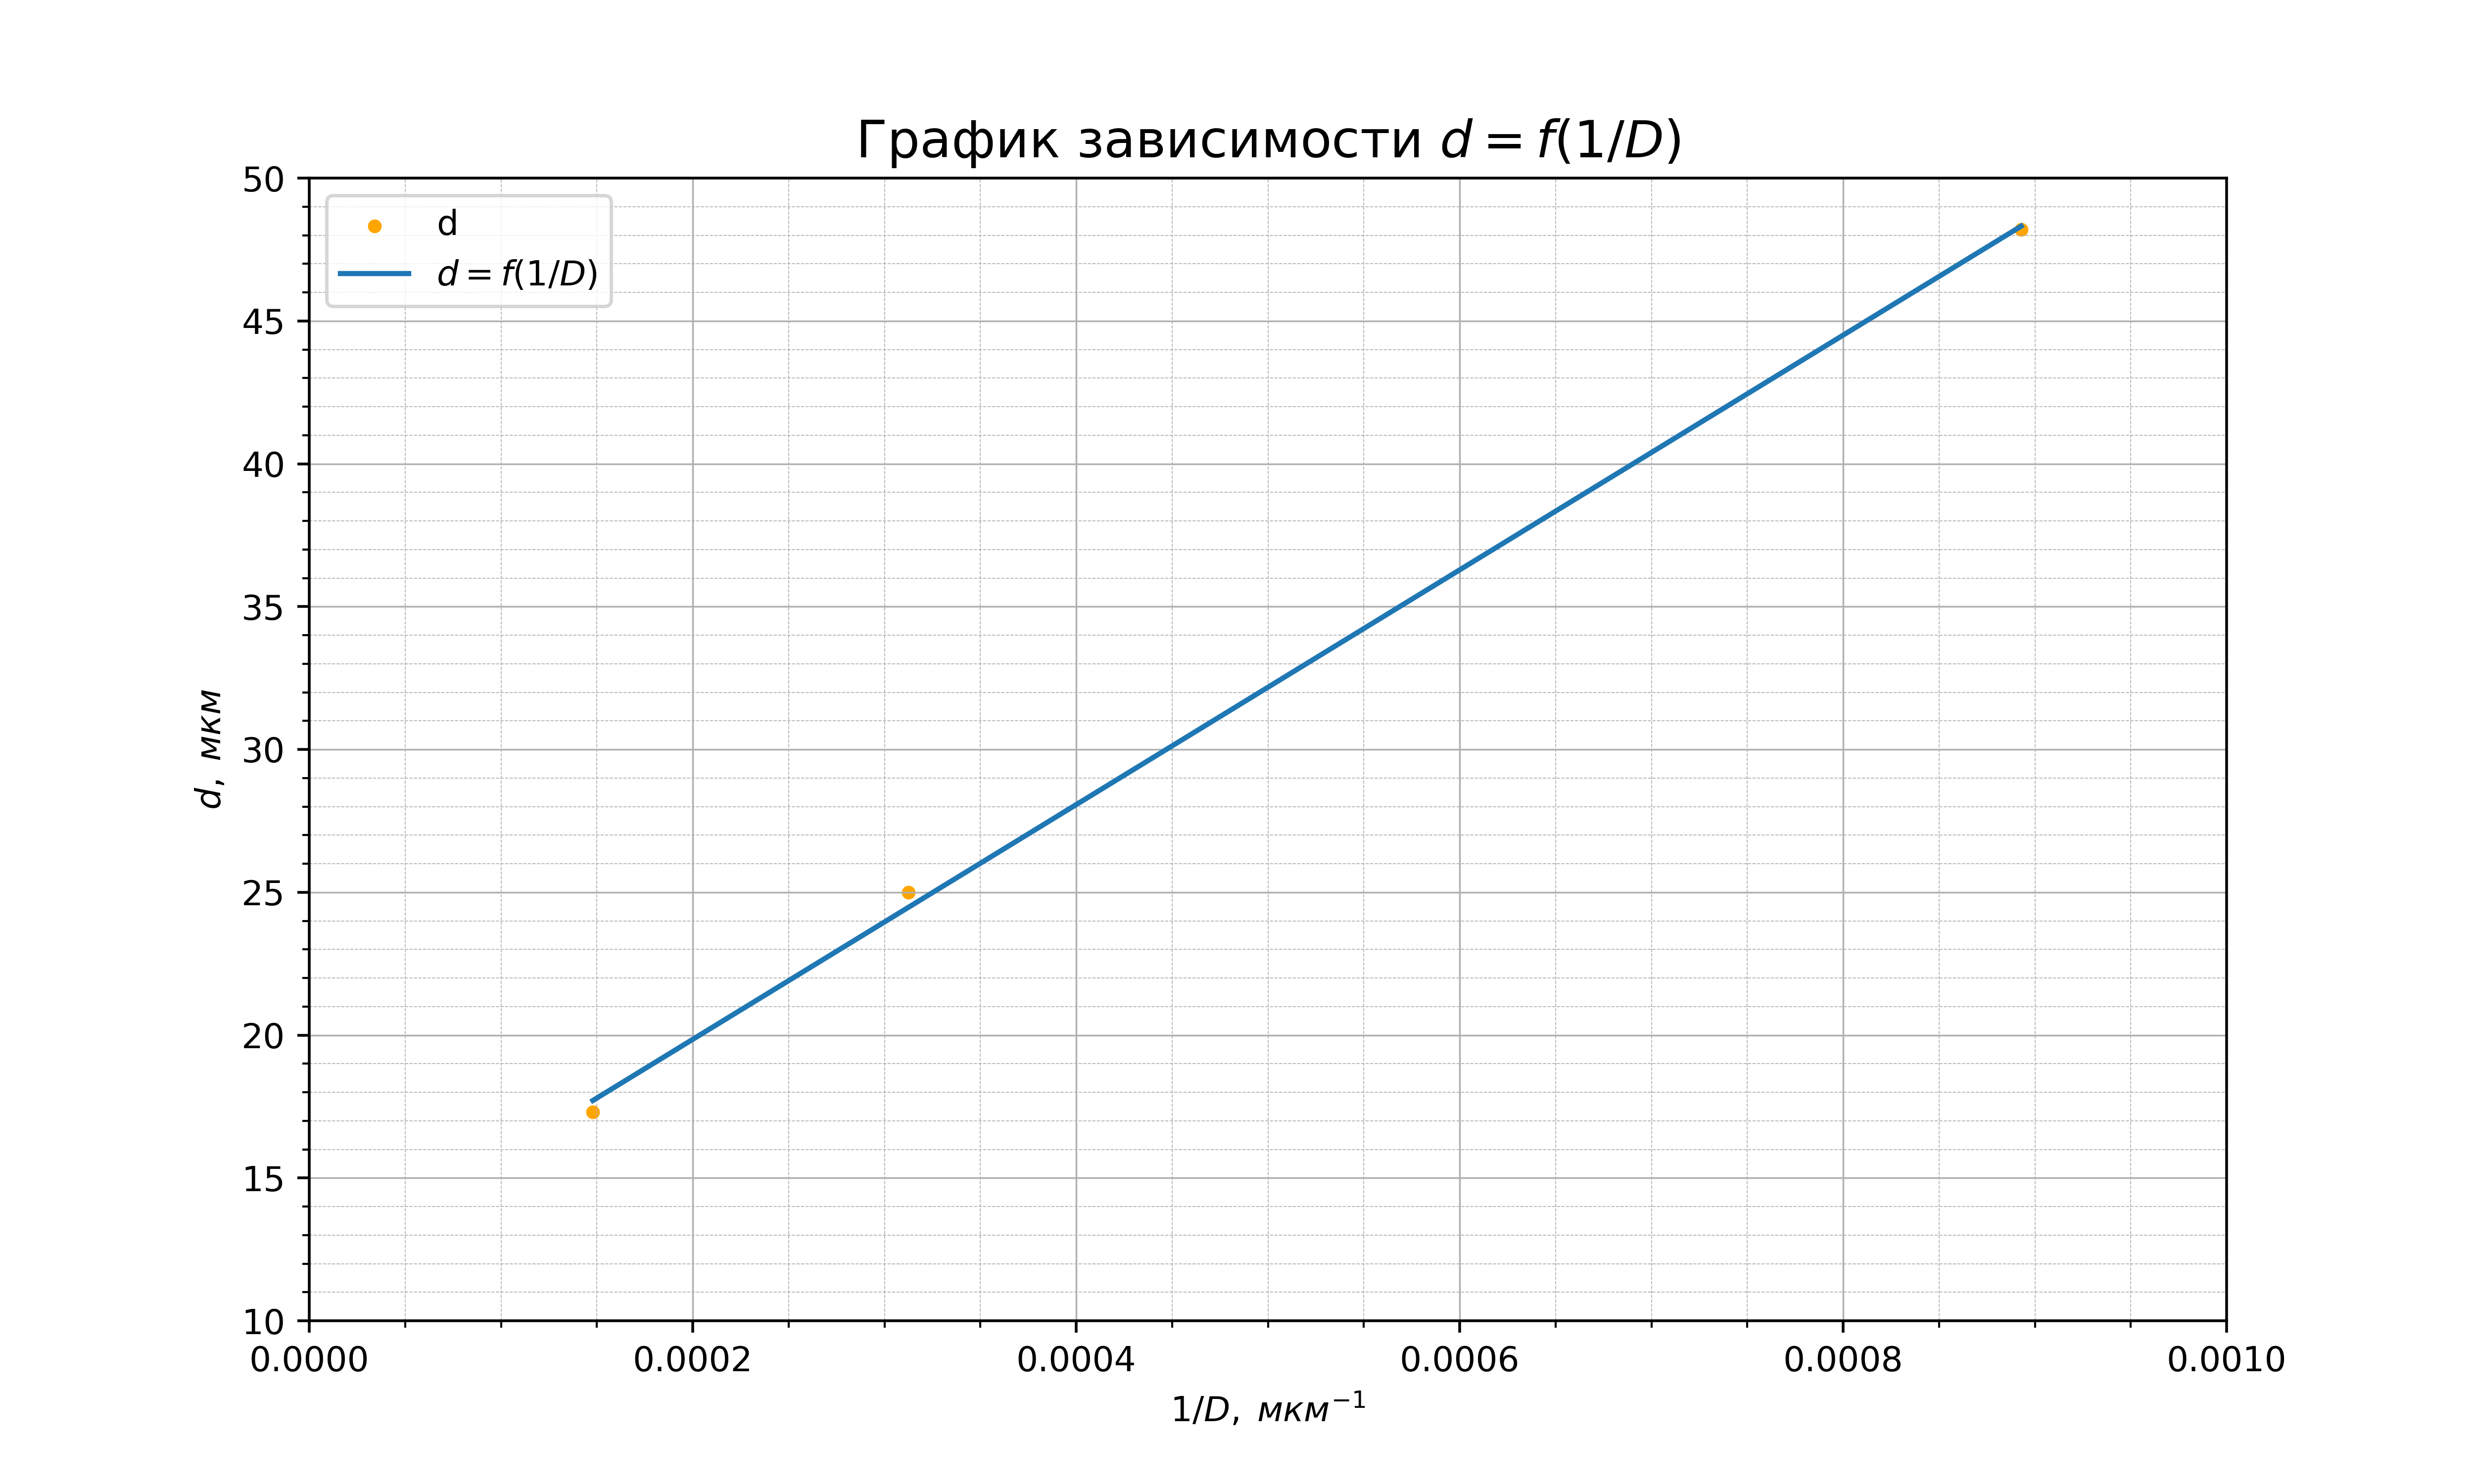
\includegraphics[scale=0.7]{4.3.3_1.png}
\end{center}
\caption{График зависимости периода решётки от минимального размера диафрагмы}
\label{plot:Abbe}
\end{figure}

\newpage

\subsection{Пространственная фильтрация и мультиплицирование}

Поворачивая щель относительно оси системы, получим изображения решёток при различных ориентациях щели. Для вертикального и горизонтального положения, когда видны только соответствующие дифракционные максимумы, получаем период $l \approx 3~мм$. Для наклонного положения решётки под углом $45^{\circ}$, когда пропускаются максимумы с $m_x = m_y$, получим $l \approx 2~мм$, т. е. меньше в $\sqrt{2}$ раз. Это объясняется тем, что расстояние между вторичными источниками волн составляет $\frac{d}{\sqrt{2}}$.

Для наблюдения мультиплицирования поменяем местами сетку и щель. Подберём такую ширину щели, чтобы на экране можно было наблюдать мультиплицированное изображение для всех сеток. При уменьшении периода сетки период полос на экране увеличивается (рис.~\ref{fig:grid_multi1}). При увеличении ширины щели наблюдается ухудшение картины (рис.~\ref{fig:grid_multi2}).

\begin{figure}[h!]
		\begin{minipage}[h!]{0.3\linewidth}
			\center{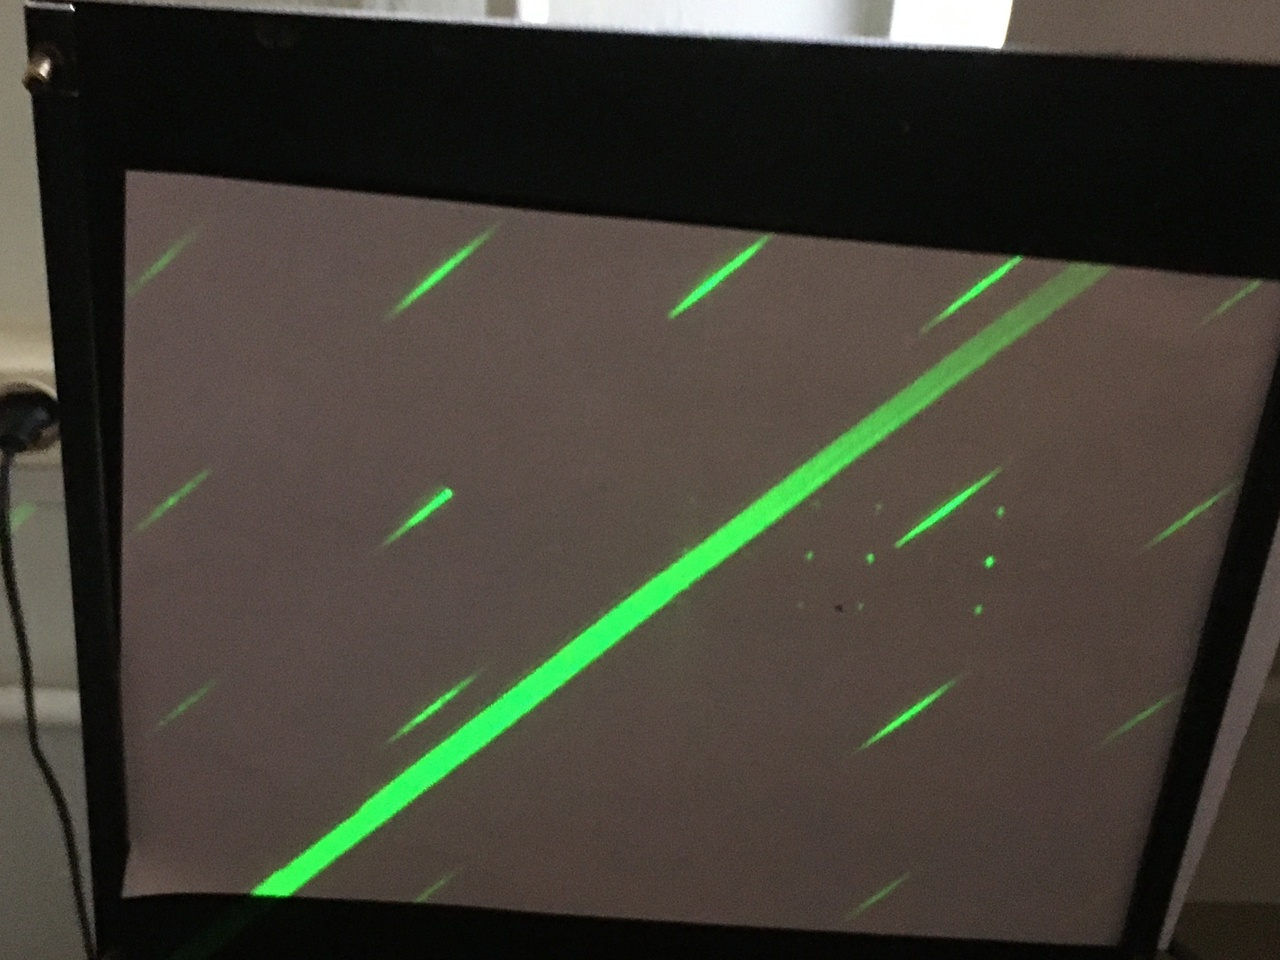
\includegraphics[width=1\linewidth]{multi1.jpg} \\ 1 решётка}
		\end{minipage}
		\hfill
		\begin{minipage}[h!]{0.3\linewidth}
			\center{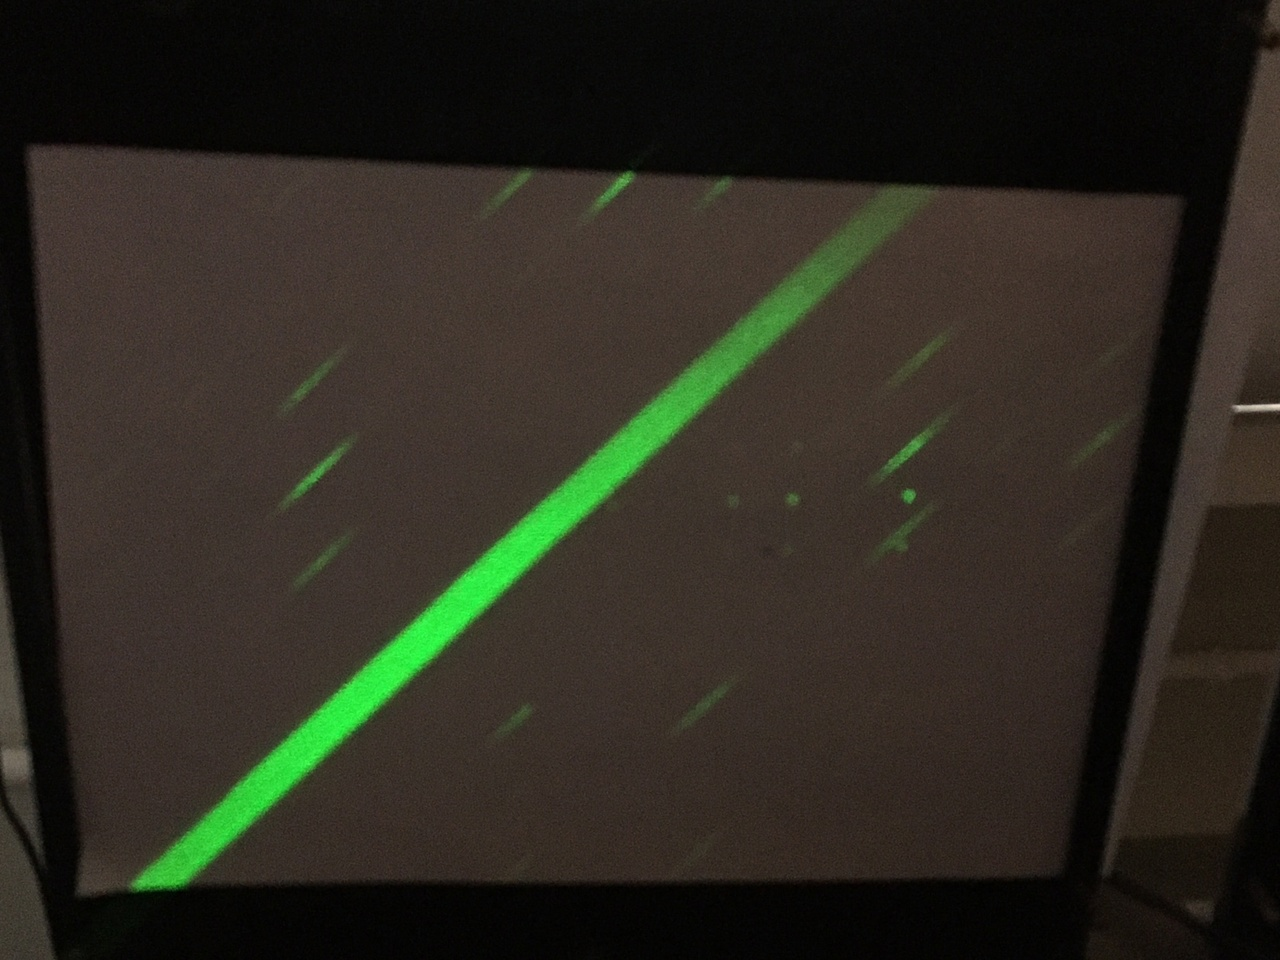
\includegraphics[width=1\linewidth]{multi2.jpg} \\ 2 решётка}
		\end{minipage}
		\hfill
		\begin{minipage}[h!]{0.3\linewidth}
			\center{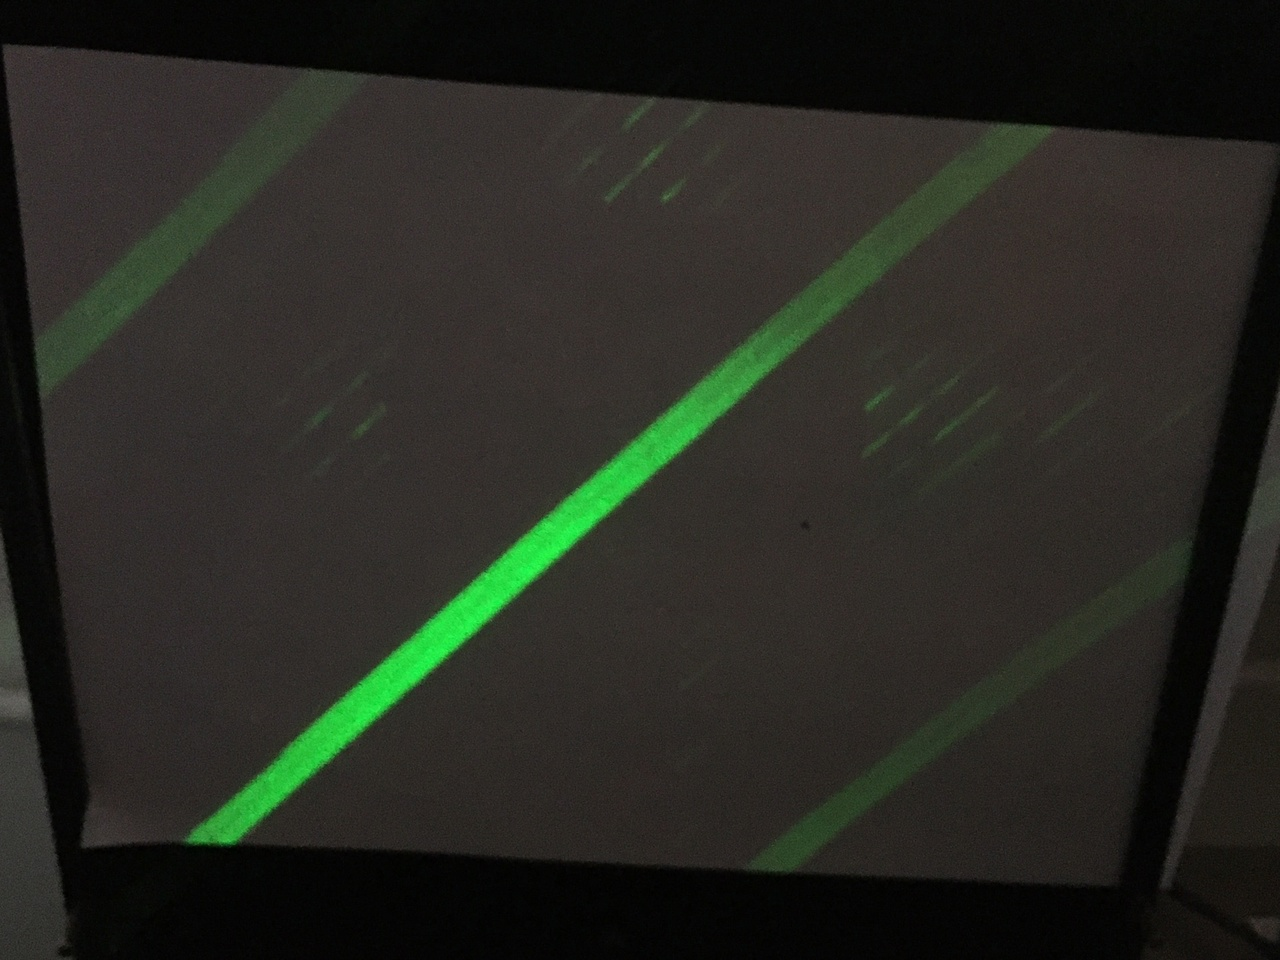
\includegraphics[width=1\linewidth]{multi3.jpg} \\ 3 решётка}
		\end{minipage}
		\hfill
		\caption{Мультиплицирование изображений дифракционных решёток}
		\label{fig:grid_multi1}
\end{figure}

\begin{figure}[h!]
		\begin{minipage}[h!]{0.3\linewidth}
			\center{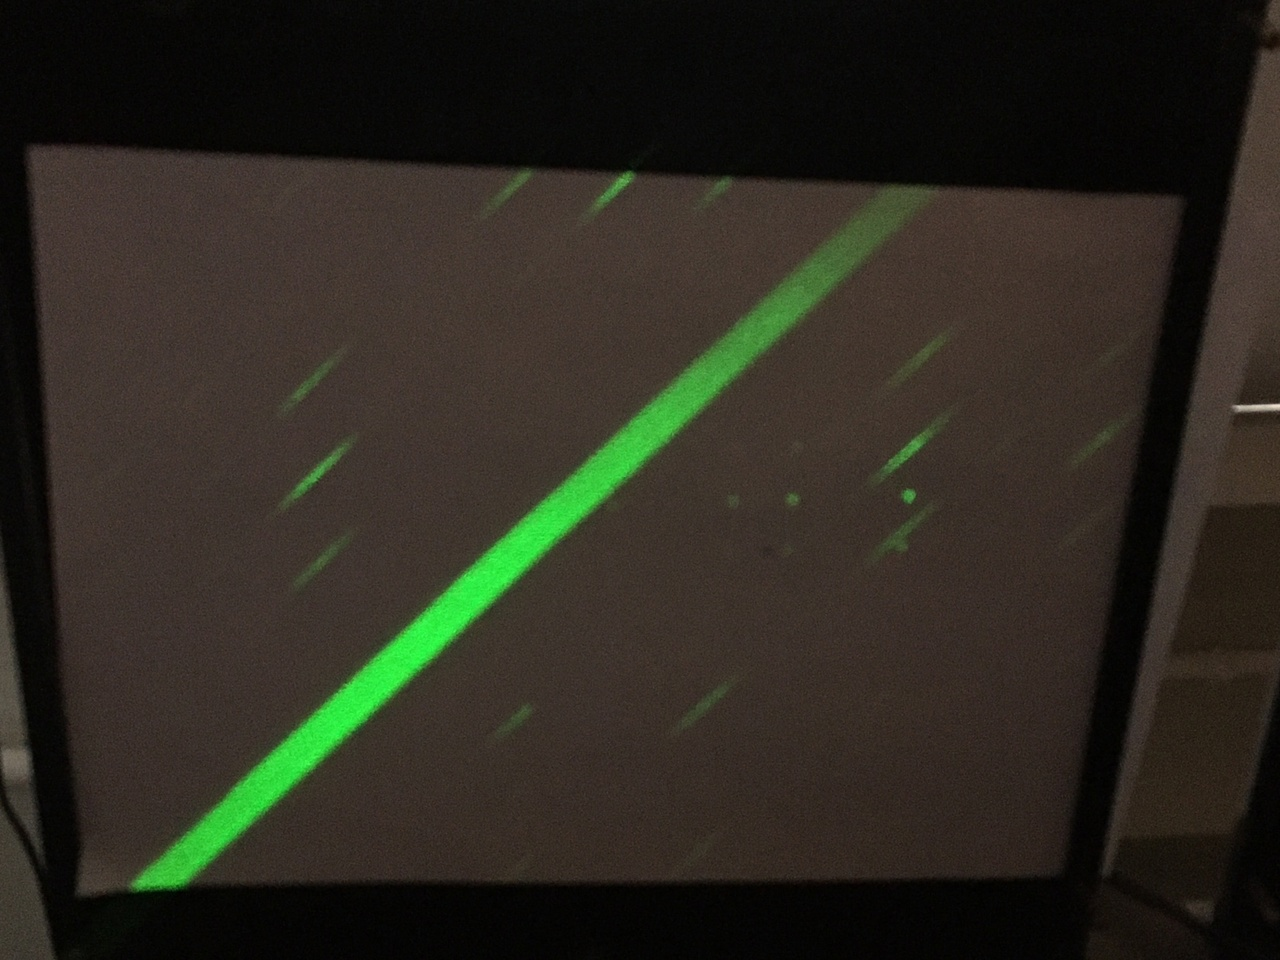
\includegraphics[width=1\linewidth]{multi2.jpg}}
		\end{minipage}
		\hfill
		\begin{minipage}[h!]{0.3\linewidth}
			\center{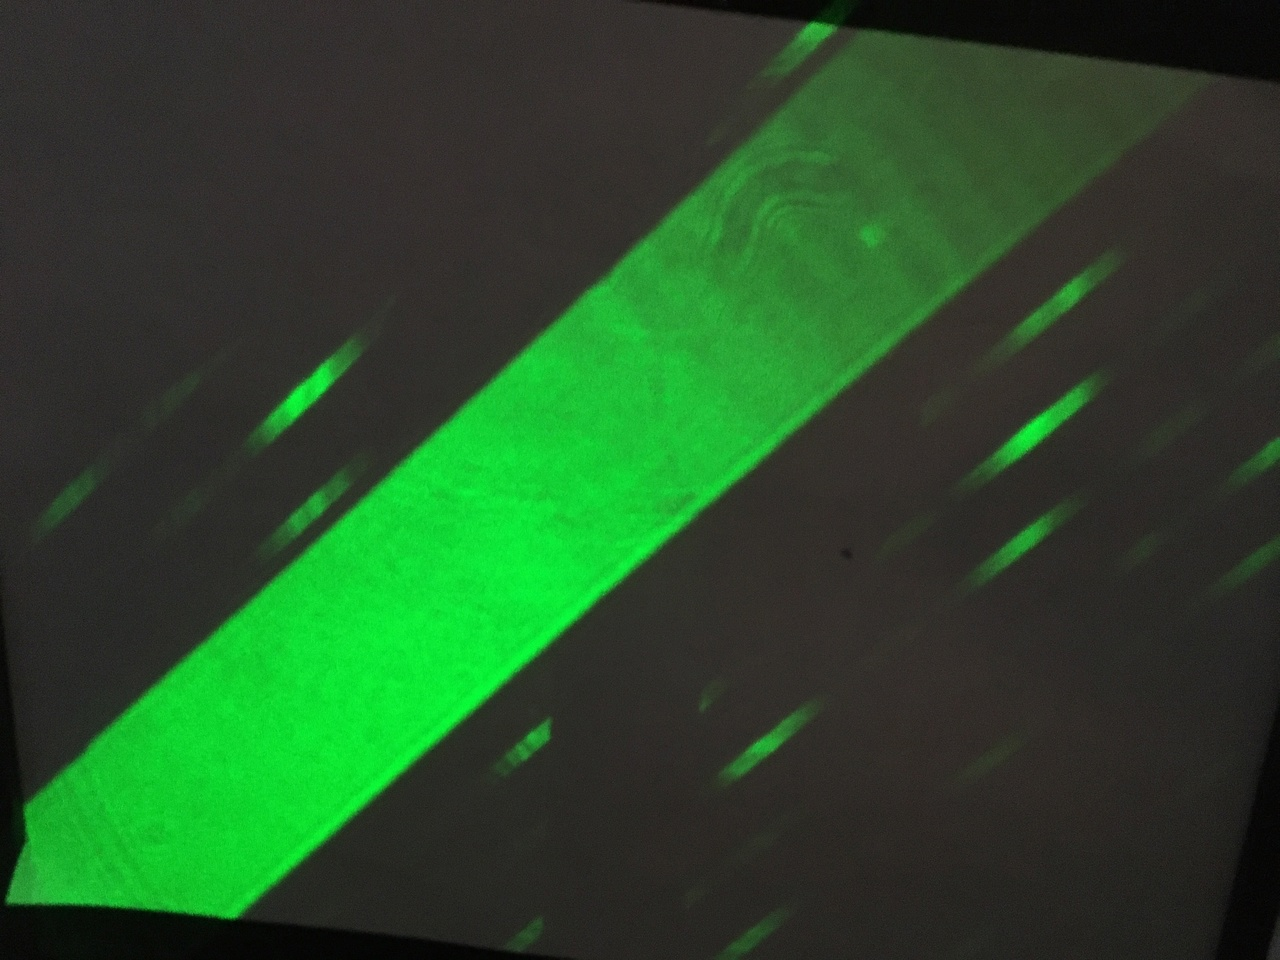
\includegraphics[width=1\linewidth]{multi4.jpg}}
		\end{minipage}
		\hfill
		\begin{minipage}[h!]{0.3\linewidth}
			\center{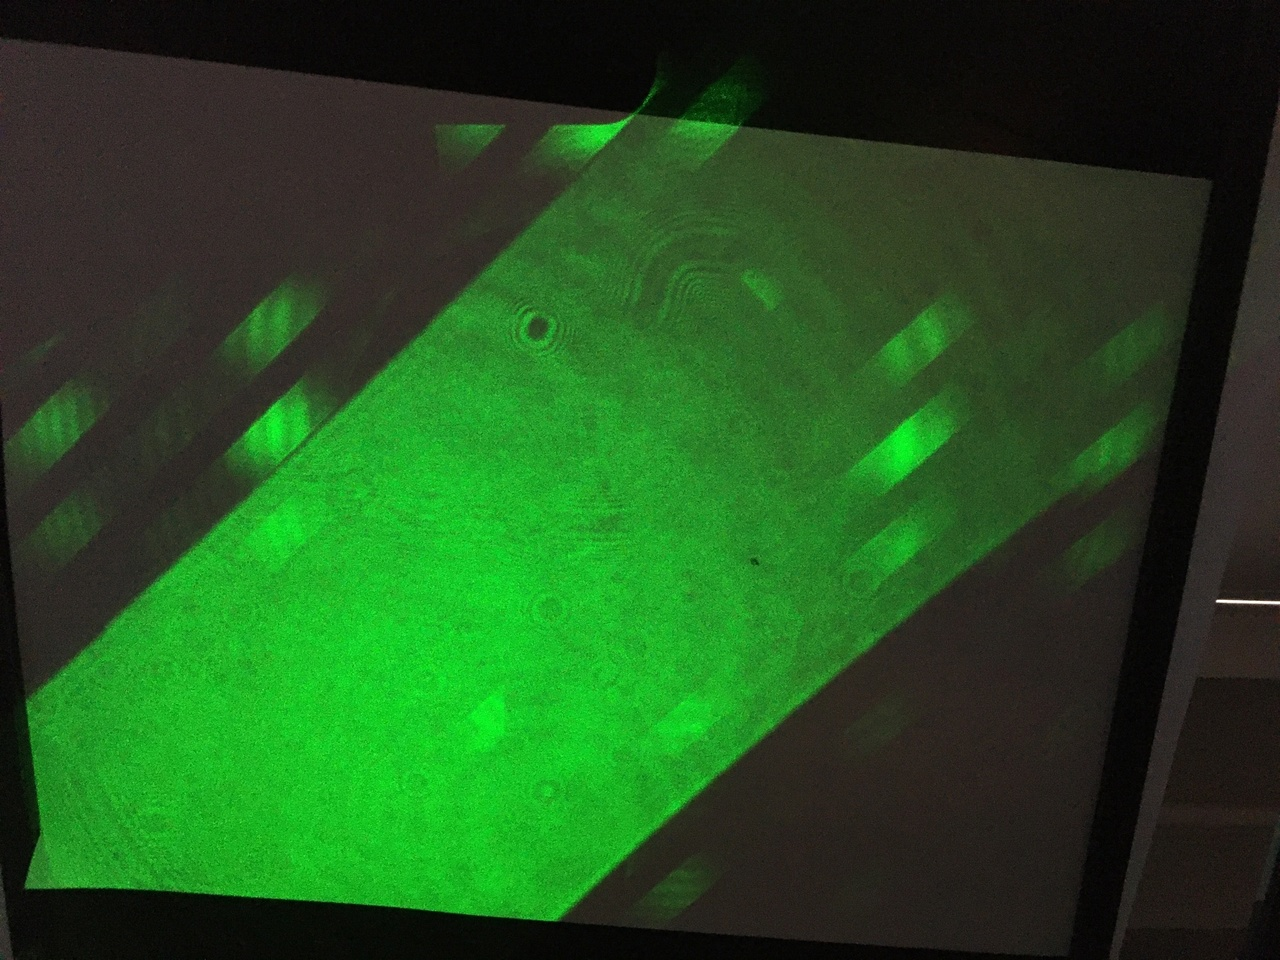
\includegraphics[width=1\linewidth]{multi5.jpg}}
		\end{minipage}
		\hfill
		\caption{Ухудшение картины при увеличении ширины щели для 2 решётки}
		\label{fig:grid_multi2}
\end{figure}

\section{Обсуждение результатов и выводы}

В данной работе были определены периоды сеток 3 разными способами: по их спектру на экране, по увеличенному с помощью модели микроскопа изображению и по результатам измерения разрешающей способности микроскопа. Результаты измерений представлены в таб.~\ref{tab:all}. Полученные значения существенно различаются, но совпадают по порядку величины. Расхождение результатов можно объяснить случайной погрешностью, связанной с точностью юстировки системы. Из графика зависимости (рис.~\ref{plot:Abbe}) $d = f(1/D)$ следует справедливость теории Аббе \eqref{min}. Также в данной работе были качественно рассмотрены явления пространственной фильтрации и мультипликации.

\end{document}
